\documentclass[twoside]{book}

% Packages required by doxygen
\usepackage{calc}
\usepackage{doxygen}
\usepackage{graphicx}
\usepackage[utf8]{inputenc}
\usepackage{makeidx}
\usepackage{multicol}
\usepackage{multirow}
\usepackage{textcomp}
\usepackage[table]{xcolor}

% Font selection
\usepackage[T1]{fontenc}
\usepackage{mathptmx}
\usepackage[scaled=.90]{helvet}
\usepackage{courier}
\usepackage{amssymb}
\usepackage{sectsty}
\renewcommand{\familydefault}{\sfdefault}
\allsectionsfont{%
  \fontseries{bc}\selectfont%
  \color{darkgray}%
}
\renewcommand{\DoxyLabelFont}{%
  \fontseries{bc}\selectfont%
  \color{darkgray}%
}

% Page & text layout
\usepackage{geometry}
\geometry{%
  a4paper,%
  top=2.5cm,%
  bottom=2.5cm,%
  left=2.5cm,%
  right=2.5cm%
}
\tolerance=750
\hfuzz=15pt
\hbadness=750
\setlength{\emergencystretch}{15pt}
\setlength{\parindent}{0cm}
\setlength{\parskip}{0.2cm}
\makeatletter
\renewcommand{\paragraph}{%
  \@startsection{paragraph}{4}{0ex}{-1.0ex}{1.0ex}{%
    \normalfont\normalsize\bfseries\SS@parafont%
  }%
}
\renewcommand{\subparagraph}{%
  \@startsection{subparagraph}{5}{0ex}{-1.0ex}{1.0ex}{%
    \normalfont\normalsize\bfseries\SS@subparafont%
  }%
}
\makeatother

% Headers & footers
\usepackage{fancyhdr}
\pagestyle{fancyplain}
\fancyhead[LE]{\fancyplain{}{\bfseries\thepage}}
\fancyhead[CE]{\fancyplain{}{}}
\fancyhead[RE]{\fancyplain{}{\bfseries\leftmark}}
\fancyhead[LO]{\fancyplain{}{\bfseries\rightmark}}
\fancyhead[CO]{\fancyplain{}{}}
\fancyhead[RO]{\fancyplain{}{\bfseries\thepage}}
\fancyfoot[LE]{\fancyplain{}{}}
\fancyfoot[CE]{\fancyplain{}{}}
\fancyfoot[RE]{\fancyplain{}{\bfseries\scriptsize Generated on Fri Feb 7 2014 19\-:15\-:08 for My Project by Doxygen }}
\fancyfoot[LO]{\fancyplain{}{\bfseries\scriptsize Generated on Fri Feb 7 2014 19\-:15\-:08 for My Project by Doxygen }}
\fancyfoot[CO]{\fancyplain{}{}}
\fancyfoot[RO]{\fancyplain{}{}}
\renewcommand{\footrulewidth}{0.4pt}
\renewcommand{\chaptermark}[1]{%
  \markboth{#1}{}%
}
\renewcommand{\sectionmark}[1]{%
  \markright{\thesection\ #1}%
}

% Indices & bibliography
\usepackage{natbib}
\usepackage[titles]{tocloft}
\setcounter{tocdepth}{3}
\setcounter{secnumdepth}{5}
\makeindex

% Hyperlinks (required, but should be loaded last)
\usepackage{ifpdf}
\ifpdf
  \usepackage[pdftex,pagebackref=true]{hyperref}
\else
  \usepackage[ps2pdf,pagebackref=true]{hyperref}
\fi
\hypersetup{%
  colorlinks=true,%
  linkcolor=blue,%
  citecolor=blue,%
  unicode%
}

% Custom commands
\newcommand{\clearemptydoublepage}{%
  \newpage{\pagestyle{empty}\cleardoublepage}%
}


%===== C O N T E N T S =====

\begin{document}

% Titlepage & ToC
\hypersetup{pageanchor=false}
\pagenumbering{roman}
\begin{titlepage}
\vspace*{7cm}
\begin{center}%
{\Large My Project }\\
\vspace*{1cm}
{\large Generated by Doxygen 1.8.6}\\
\vspace*{0.5cm}
{\small Fri Feb 7 2014 19:15:08}\\
\end{center}
\end{titlepage}
\clearemptydoublepage
\tableofcontents
\clearemptydoublepage
\pagenumbering{arabic}
\hypersetup{pageanchor=true}

%--- Begin generated contents ---
\chapter{Hierarchical Index}
\section{Class Hierarchy}
This inheritance list is sorted roughly, but not completely, alphabetically\-:\begin{DoxyCompactList}
\item \contentsline{section}{Chess\-Game\-Demo\-Test}{\pageref{class_chess_game_demo_test}}{}
\item \contentsline{section}{Game}{\pageref{class_game}}{}
\item J\-Frame\begin{DoxyCompactList}
\item \contentsline{section}{Chess\-Game\-Demo}{\pageref{class_chess_game_demo}}{}
\end{DoxyCompactList}
\item Mouse\-Listener\begin{DoxyCompactList}
\item \contentsline{section}{Chess\-Game\-Demo}{\pageref{class_chess_game_demo}}{}
\end{DoxyCompactList}
\item Mouse\-Motion\-Listener\begin{DoxyCompactList}
\item \contentsline{section}{Chess\-Game\-Demo}{\pageref{class_chess_game_demo}}{}
\end{DoxyCompactList}
\item \contentsline{section}{Movement\-Check}{\pageref{class_movement_check}}{}
\item \contentsline{section}{Movement\-Check\-Test}{\pageref{class_movement_check_test}}{}
\end{DoxyCompactList}

\chapter{Class Index}
\section{Class List}
Here are the classes, structs, unions and interfaces with brief descriptions\-:\begin{DoxyCompactList}
\item\contentsline{section}{\hyperlink{class_chess_game_demo}{Chess\-Game\-Demo} }{\pageref{class_chess_game_demo}}{}
\item\contentsline{section}{\hyperlink{class_chess_game_demo_test}{Chess\-Game\-Demo\-Test} }{\pageref{class_chess_game_demo_test}}{}
\item\contentsline{section}{\hyperlink{class_game}{Game} }{\pageref{class_game}}{}
\item\contentsline{section}{\hyperlink{class_movement_1_1_movement}{Movement.\-Movement} }{\pageref{class_movement_1_1_movement}}{}
\item\contentsline{section}{\hyperlink{class_movement_1_1_movement_bishop}{Movement.\-Movement\-Bishop} }{\pageref{class_movement_1_1_movement_bishop}}{}
\item\contentsline{section}{\hyperlink{class_movement_test_1_1_movement_bishop_test}{Movement\-Test.\-Movement\-Bishop\-Test} }{\pageref{class_movement_test_1_1_movement_bishop_test}}{}
\item\contentsline{section}{\hyperlink{class_movement_check}{Movement\-Check} }{\pageref{class_movement_check}}{}
\item\contentsline{section}{\hyperlink{class_movement_check_test}{Movement\-Check\-Test} }{\pageref{class_movement_check_test}}{}
\item\contentsline{section}{\hyperlink{class_movement_1_1_movement_king}{Movement.\-Movement\-King} }{\pageref{class_movement_1_1_movement_king}}{}
\item\contentsline{section}{\hyperlink{class_movement_test_1_1_movement_king_test}{Movement\-Test.\-Movement\-King\-Test} }{\pageref{class_movement_test_1_1_movement_king_test}}{}
\item\contentsline{section}{\hyperlink{class_movement_1_1_movement_knight}{Movement.\-Movement\-Knight} }{\pageref{class_movement_1_1_movement_knight}}{}
\item\contentsline{section}{\hyperlink{class_movement_test_1_1_movement_knight_test}{Movement\-Test.\-Movement\-Knight\-Test} }{\pageref{class_movement_test_1_1_movement_knight_test}}{}
\item\contentsline{section}{\hyperlink{class_movement_1_1_movement_pawn}{Movement.\-Movement\-Pawn} }{\pageref{class_movement_1_1_movement_pawn}}{}
\item\contentsline{section}{\hyperlink{class_movement_test_1_1_movement_pawn_test}{Movement\-Test.\-Movement\-Pawn\-Test} }{\pageref{class_movement_test_1_1_movement_pawn_test}}{}
\item\contentsline{section}{\hyperlink{class_movement_1_1_movement_rock}{Movement.\-Movement\-Rock} }{\pageref{class_movement_1_1_movement_rock}}{}
\item\contentsline{section}{\hyperlink{class_basic___objects_1_1_piece}{Basic\-\_\-\-Objects.\-Piece} }{\pageref{class_basic___objects_1_1_piece}}{}
\item\contentsline{section}{\hyperlink{class_basic___objects_1_1_position}{Basic\-\_\-\-Objects.\-Position} }{\pageref{class_basic___objects_1_1_position}}{}
\end{DoxyCompactList}

\chapter{Class Documentation}
\hypertarget{class_chess_game_demo}{\section{Chess\-Game\-Demo Class Reference}
\label{class_chess_game_demo}\index{Chess\-Game\-Demo@{Chess\-Game\-Demo}}
}
Inheritance diagram for Chess\-Game\-Demo\-:\begin{figure}[H]
\begin{center}
\leavevmode
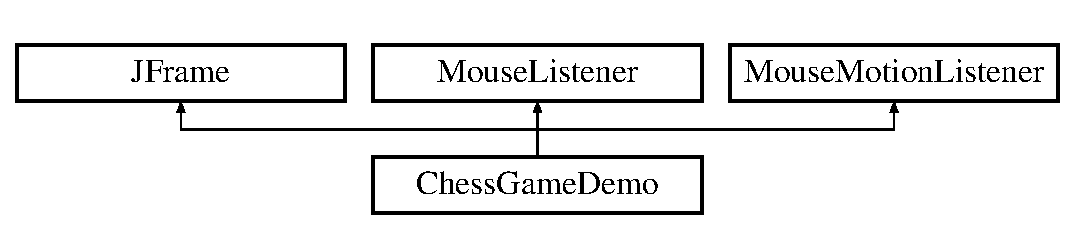
\includegraphics[height=2.000000cm]{class_chess_game_demo}
\end{center}
\end{figure}
\subsection*{Public Member Functions}
\begin{DoxyCompactItemize}
\item 
\hypertarget{class_chess_game_demo_ab52c4364333b4e4ec27bd731c7b2256f}{void {\bfseries mouse\-Pressed} (Mouse\-Event e)}\label{class_chess_game_demo_ab52c4364333b4e4ec27bd731c7b2256f}

\item 
\hypertarget{class_chess_game_demo_a20232f9f79c24183355215d5d9fb97f8}{void {\bfseries mouse\-Dragged} (Mouse\-Event me)}\label{class_chess_game_demo_a20232f9f79c24183355215d5d9fb97f8}

\item 
\hypertarget{class_chess_game_demo_a4ed6a1f2ef893a991284314aff24ccdd}{void {\bfseries mouse\-Released} (Mouse\-Event e)}\label{class_chess_game_demo_a4ed6a1f2ef893a991284314aff24ccdd}

\item 
\hypertarget{class_chess_game_demo_a72b1027bb8e3c6e29a098408e0e800f6}{Boolean {\bfseries get\-Finish} ()}\label{class_chess_game_demo_a72b1027bb8e3c6e29a098408e0e800f6}

\item 
\hypertarget{class_chess_game_demo_a004e02ac96f039240269badbf2d08b8c}{void {\bfseries mouse\-Clicked} (Mouse\-Event e)}\label{class_chess_game_demo_a004e02ac96f039240269badbf2d08b8c}

\item 
\hypertarget{class_chess_game_demo_a91cb907f923dafdfc2e98b4a0d64f608}{void {\bfseries mouse\-Moved} (Mouse\-Event e)}\label{class_chess_game_demo_a91cb907f923dafdfc2e98b4a0d64f608}

\item 
\hypertarget{class_chess_game_demo_a5adfb134fa4f1f85c234fac389408eca}{void {\bfseries mouse\-Entered} (Mouse\-Event e)}\label{class_chess_game_demo_a5adfb134fa4f1f85c234fac389408eca}

\item 
\hypertarget{class_chess_game_demo_a37c5d938478f8ff26d889db218343cb9}{void {\bfseries mouse\-Exited} (Mouse\-Event e)}\label{class_chess_game_demo_a37c5d938478f8ff26d889db218343cb9}

\end{DoxyCompactItemize}


The documentation for this class was generated from the following file\-:\begin{DoxyCompactItemize}
\item 
src/Chess\-Game\-Demo.\-java\end{DoxyCompactItemize}

\hypertarget{class_chess_game_demo_test}{\section{Chess\-Game\-Demo\-Test Class Reference}
\label{class_chess_game_demo_test}\index{Chess\-Game\-Demo\-Test@{Chess\-Game\-Demo\-Test}}
}
\subsection*{Public Member Functions}
\begin{DoxyCompactItemize}
\item 
\hypertarget{class_chess_game_demo_test_ac92ec040d29bab38c5fd83ebaf19d9f9}{void {\bfseries test} ()}\label{class_chess_game_demo_test_ac92ec040d29bab38c5fd83ebaf19d9f9}

\end{DoxyCompactItemize}


The documentation for this class was generated from the following file\-:\begin{DoxyCompactItemize}
\item 
src/Chess\-Game\-Demo\-Test.\-java\end{DoxyCompactItemize}

\hypertarget{class_game}{\section{Game Class Reference}
\label{class_game}\index{Game@{Game}}
}
\subsection*{Static Public Member Functions}
\begin{DoxyCompactItemize}
\item 
\hypertarget{class_game_ae52595a27ac1b327b05db2129ad81fca}{static void {\bfseries main} (String\mbox{[}$\,$\mbox{]} args)}\label{class_game_ae52595a27ac1b327b05db2129ad81fca}

\end{DoxyCompactItemize}


The documentation for this class was generated from the following file\-:\begin{DoxyCompactItemize}
\item 
Game.\-java\end{DoxyCompactItemize}

\hypertarget{class_movement_check}{\section{Movement\-Check Class Reference}
\label{class_movement_check}\index{Movement\-Check@{Movement\-Check}}
}
\subsection*{Public Member Functions}
\begin{DoxyCompactItemize}
\item 
\hypertarget{class_movement_check_ad4282505567223574aad557238ec3962}{void {\bfseries update} (\hyperlink{class_basic___objects_1_1_piece}{Piece}\mbox{[}$\,$\mbox{]}\mbox{[}$\,$\mbox{]} \-\_\-pieces)}\label{class_movement_check_ad4282505567223574aad557238ec3962}

\item 
\hypertarget{class_movement_check_a7de16c5e5e34bea53f45a84c0357b3cf}{boolean {\bfseries check\-Move} (\hyperlink{class_basic___objects_1_1_piece}{Piece} p, \hyperlink{class_basic___objects_1_1_position}{Position} \-\_\-init, \hyperlink{class_basic___objects_1_1_position}{Position} \-\_\-end)}\label{class_movement_check_a7de16c5e5e34bea53f45a84c0357b3cf}

\item 
\hypertarget{class_movement_check_a419c5a5eba3dd02a9a9d0fe56df331b9}{boolean {\bfseries check} (\hyperlink{class_basic___objects_1_1_position}{Position} \-\_\-end, boolean Color)}\label{class_movement_check_a419c5a5eba3dd02a9a9d0fe56df331b9}

\item 
\hypertarget{class_movement_check_a6f044b7c75dd4d54dc1253937e885c6a}{boolean {\bfseries check\-Mate} (boolean Color)}\label{class_movement_check_a6f044b7c75dd4d54dc1253937e885c6a}

\end{DoxyCompactItemize}


The documentation for this class was generated from the following file\-:\begin{DoxyCompactItemize}
\item 
src/Movement\-Check.\-java\end{DoxyCompactItemize}

\hypertarget{class_movement_check_test}{\section{Movement\-Check\-Test Class Reference}
\label{class_movement_check_test}\index{Movement\-Check\-Test@{Movement\-Check\-Test}}
}
\subsection*{Public Member Functions}
\begin{DoxyCompactItemize}
\item 
void \hyperlink{class_movement_check_test_ad2909b021508f999bffedc9dc744a737}{test\-Exception\-Is\-Thrown} ()
\item 
void \hyperlink{class_movement_check_test_af9b5c9b924d8d81b1e298aee638f8f77}{test\-Check\-Move} ()
\item 
void \hyperlink{class_movement_check_test_a701b7fb280075841f2deac18bc41eb86}{test\-Check} ()
\item 
void \hyperlink{class_movement_check_test_a06f6f6fa710f8177f2f8d3eb047ebe7c}{test\-Check\-Mate} ()
\end{DoxyCompactItemize}


\subsection{Detailed Description}
\begin{DoxyAuthor}{Author}
ignacioferrero 
\end{DoxyAuthor}


\subsection{Member Function Documentation}
\hypertarget{class_movement_check_test_a701b7fb280075841f2deac18bc41eb86}{\index{Movement\-Check\-Test@{Movement\-Check\-Test}!test\-Check@{test\-Check}}
\index{test\-Check@{test\-Check}!MovementCheckTest@{Movement\-Check\-Test}}
\subsubsection[{test\-Check}]{\setlength{\rightskip}{0pt plus 5cm}void Movement\-Check\-Test.\-test\-Check (
\begin{DoxyParamCaption}
{}
\end{DoxyParamCaption}
)}}\label{class_movement_check_test_a701b7fb280075841f2deac18bc41eb86}
Test method for \hyperlink{}{Movement\-Check\#check(\-Position, boolean)}. \hypertarget{class_movement_check_test_a06f6f6fa710f8177f2f8d3eb047ebe7c}{\index{Movement\-Check\-Test@{Movement\-Check\-Test}!test\-Check\-Mate@{test\-Check\-Mate}}
\index{test\-Check\-Mate@{test\-Check\-Mate}!MovementCheckTest@{Movement\-Check\-Test}}
\subsubsection[{test\-Check\-Mate}]{\setlength{\rightskip}{0pt plus 5cm}void Movement\-Check\-Test.\-test\-Check\-Mate (
\begin{DoxyParamCaption}
{}
\end{DoxyParamCaption}
)}}\label{class_movement_check_test_a06f6f6fa710f8177f2f8d3eb047ebe7c}
Test method for \hyperlink{}{Movement\-Check\#check\-Mate(boolean)}. \hypertarget{class_movement_check_test_af9b5c9b924d8d81b1e298aee638f8f77}{\index{Movement\-Check\-Test@{Movement\-Check\-Test}!test\-Check\-Move@{test\-Check\-Move}}
\index{test\-Check\-Move@{test\-Check\-Move}!MovementCheckTest@{Movement\-Check\-Test}}
\subsubsection[{test\-Check\-Move}]{\setlength{\rightskip}{0pt plus 5cm}void Movement\-Check\-Test.\-test\-Check\-Move (
\begin{DoxyParamCaption}
{}
\end{DoxyParamCaption}
)}}\label{class_movement_check_test_af9b5c9b924d8d81b1e298aee638f8f77}
Test method for \hyperlink{}{Movement\-Check\#check\-Move(\-Piece, Position, Position)}. \hypertarget{class_movement_check_test_ad2909b021508f999bffedc9dc744a737}{\index{Movement\-Check\-Test@{Movement\-Check\-Test}!test\-Exception\-Is\-Thrown@{test\-Exception\-Is\-Thrown}}
\index{test\-Exception\-Is\-Thrown@{test\-Exception\-Is\-Thrown}!MovementCheckTest@{Movement\-Check\-Test}}
\subsubsection[{test\-Exception\-Is\-Thrown}]{\setlength{\rightskip}{0pt plus 5cm}void Movement\-Check\-Test.\-test\-Exception\-Is\-Thrown (
\begin{DoxyParamCaption}
{}
\end{DoxyParamCaption}
)}}\label{class_movement_check_test_ad2909b021508f999bffedc9dc744a737}
Test method for \hyperlink{}{Movement\-Check\#update(\-Piece\mbox{[}$\,$\mbox{]}\mbox{[}$\,$\mbox{]})}. 

The documentation for this class was generated from the following file\-:\begin{DoxyCompactItemize}
\item 
Movement\-Check\-Test.\-java\end{DoxyCompactItemize}

%--- End generated contents ---

% Index
\newpage
\phantomsection
\addcontentsline{toc}{chapter}{Index}
\printindex

\end{document}
